% =====================================================================
%  Reinforcement Learning Assignment — 3MD3220, CentraleSupélec 2026
%  Springer LNCS template  |  Max 3 pages excl. references & figures
% =====================================================================
\documentclass[runningheads]{llncs}

\usepackage[T1]{fontenc}
\usepackage[utf8]{inputenc}
\usepackage{graphicx}
\usepackage{amsmath}
\usepackage{booktabs}
\usepackage{hyperref}
\usepackage{float}
\usepackage{xcolor}

\hypersetup{colorlinks=true,linkcolor=blue!60!black,
            citecolor=blue!60!black,urlcolor=blue!60!black}

% tighten list spacing globally
\usepackage{enumitem}
\setlist[itemize]{nosep,leftmargin=*}
\setlist[enumerate]{nosep,leftmargin=*}

\begin{document}

% ------------------------------------------------------------------
\title{Comparing First-Visit Monte Carlo and Sarsa($\lambda$)\\
       on Text Flappy Bird}

\author{Julian}
\authorrunning{Julian}
\institute{CentraleSupélec — 3MD3220 Reinforcement Learning, April 2026}

\maketitle

% ------------------------------------------------------------------
\begin{abstract}
We implement and compare two tabular reinforcement learning agents —
First-Visit Monte Carlo (MC) and Sarsa($\lambda$) — on the
\texttt{TextFlappyBird-v0} environment.
After 25\,000 training episodes Sarsa($\lambda$) achieves a mean score of
\textbf{199 pipes} vs.\ \textbf{65 pipes} for MC, demonstrating the advantage
of online, trace-based updates.
We report learning curves, value-function heatmaps, policy maps, parameter
sweeps, and a generalisation study across environment configurations.
\end{abstract}

% ------------------------------------------------------------------
\section{Experimental Setup}

\textbf{Environment.}
\texttt{TextFlappyBird-v0}~\cite{christodoulidis2023tfb} returns a 2-tuple
$(x_\text{dist}, y_\text{dist})$ — the player's horizontal and vertical
distance to the nearest pipe gap.
With the default config (\texttt{height}=15, \texttt{width}=20,
\texttt{pipe\_gap}=4) the discrete state space contains $14\!\times\!22=308$
states; the action space is binary ($0=\text{idle}$, $1=\text{flap}$).
Every step survived gives reward $+1$; episodes terminate on collision or
after 2\,000 steps.

\textbf{Hyperparameters.}
Both agents share: $\alpha=0.1$, $\gamma=0.99$, initial
$\varepsilon=0.1$ (decaying to $0.01$), 25\,000 episodes.
Sarsa additionally uses $\lambda=0.7$.

% ------------------------------------------------------------------
\section{Agent Implementations}

\textbf{First-Visit MC.}
MC collects a full episode, then updates Q only at the \emph{first} visit to
each $(S_t,A_t)$:
\[
  Q(S_t,A_t) \leftarrow Q(S_t,A_t)+\alpha\!\left[G_t - Q(S_t,A_t)\right],
  \quad G_t=\sum_{k=0}^{T-t-1}\gamma^k R_{t+k+1}.
\]
No bootstrapping is used, so updates are unbiased but high-variance.

\textbf{Sarsa($\lambda$)~\cite{sutton2018rl}.}
At every step Sarsa computes a TD-error $\delta_t$ and propagates credit
via eligibility traces $E(s,a)$:
\begin{align*}
  \delta_t &= R_{t+1}+\gamma Q(S_{t+1},A_{t+1})-Q(S_t,A_t),\\
  E(S_t,A_t) &\leftarrow E(S_t,A_t)+1,\\
  Q(s,a) &\leftarrow Q(s,a)+\alpha\,\delta_t\,E(s,a),\quad
  E(s,a) \leftarrow \gamma\lambda\,E(s,a).
\end{align*}
Online updates and multi-step credit assignment lead to much faster convergence.

% ------------------------------------------------------------------
\section{Results}

\textbf{Learning curves (Fig.~\ref{fig:curves}).}
Sarsa($\lambda$) (teal) rises steeply and plateaus near 2\,000
reward steps around episode 15\,000.
MC (orange) converges slowly with high variance, consistent with its
end-of-episode, no-bootstrapping design.
Final greedy evaluation over 500 episodes:
\textbf{Sarsa 199.0 pipes / 2\,000 steps} vs.\ \textbf{MC 65.2 pipes / 662 steps}.

\textbf{Value functions (Fig.~\ref{fig:value}).}
Both agents learn that small $|y_\text{dist}|$ (vertically aligned with the gap)
is highly valuable. Sarsa's heatmap is smoother and more complete (298/308 states
visited vs.\ 271/308 for MC), reflecting better credit propagation.

\textbf{Policy maps (Fig.~\ref{fig:policy}).}
Both agents converge to the intuitive strategy:
\emph{flap} when below the gap ($y_\text{dist}>0$), \emph{idle} when above.
Sarsa covers nearly every state; MC leaves corner states at default Q~=~0.

% -------  Figures (excluded from 3-page count) --------------------
\begin{figure}[H]
  \centering
  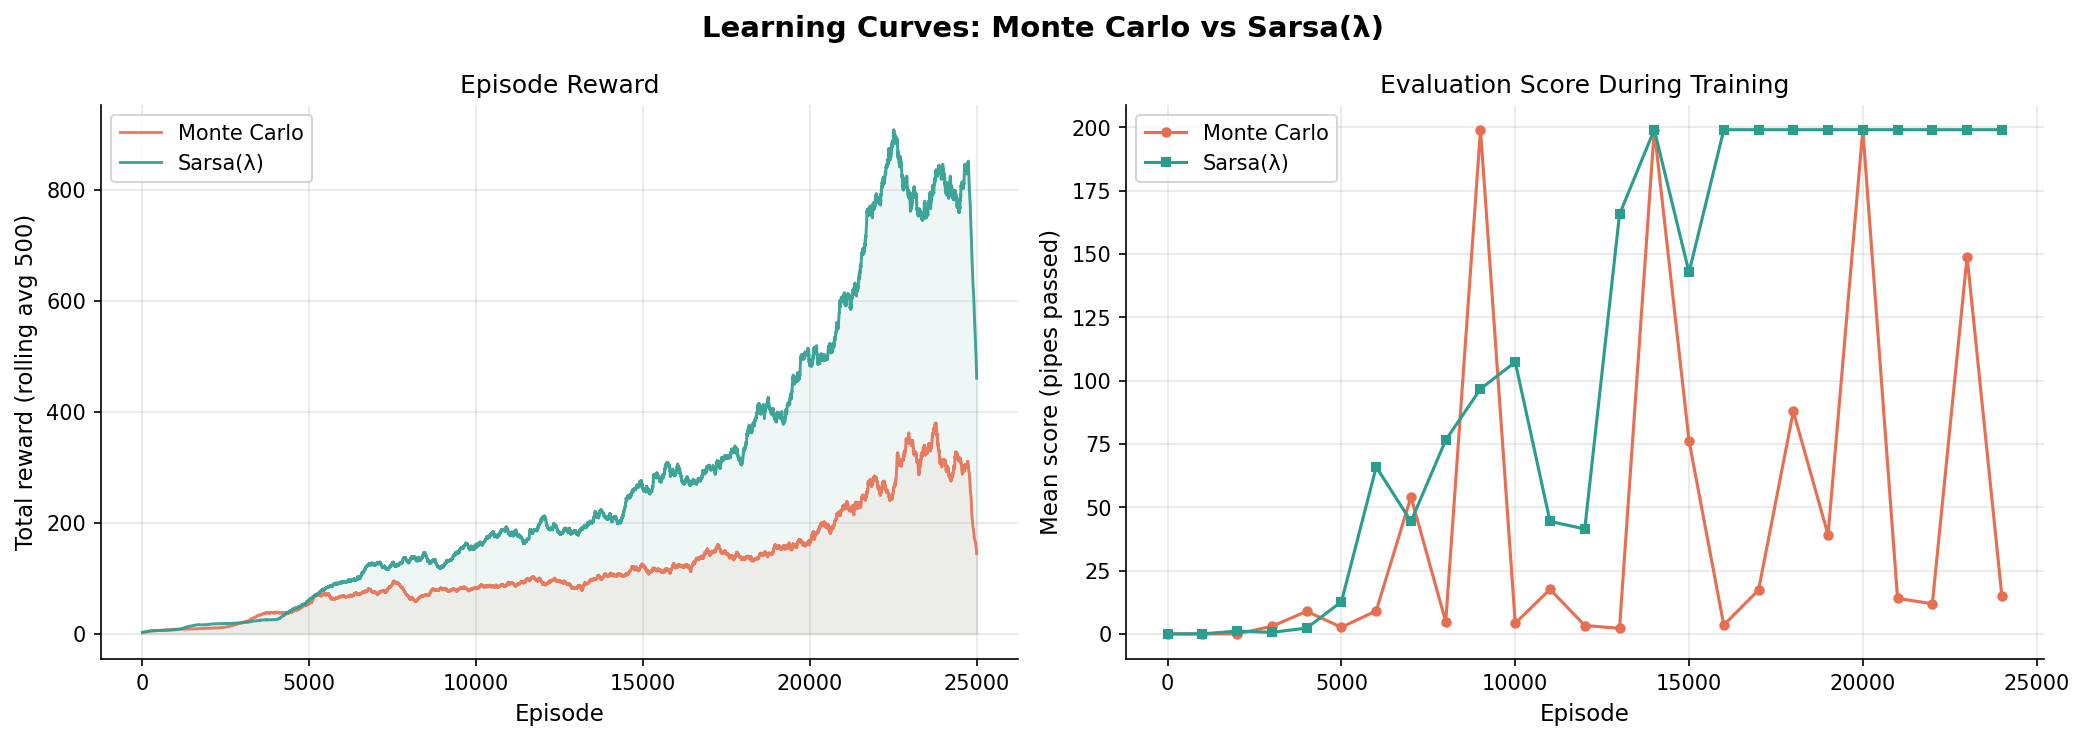
\includegraphics[width=\linewidth]{learning_curves.png}
  \caption{Learning curves: rolling reward (left) and pipe score (right)
           over 25\,000 episodes.}
  \label{fig:curves}
\end{figure}

\begin{figure}[H]
  \centering
  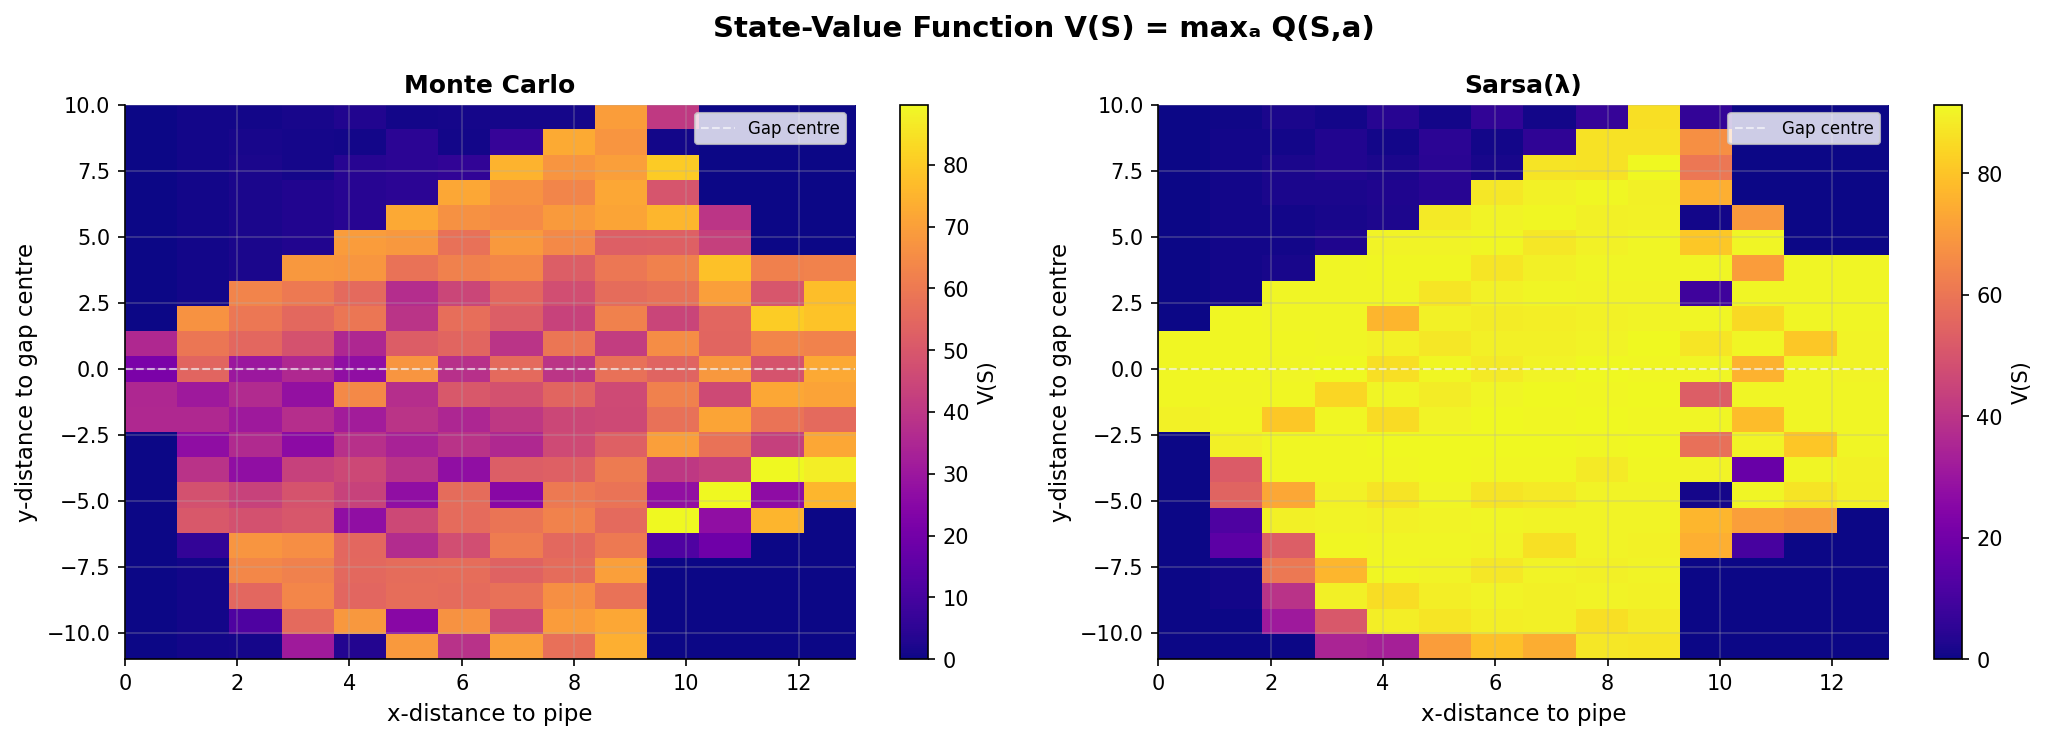
\includegraphics[width=\linewidth]{value_functions.png}
  \caption{State-value heatmaps $V(s)=\max_a Q(s,a)$.}
  \label{fig:value}
\end{figure}

\begin{figure}[H]
  \centering
  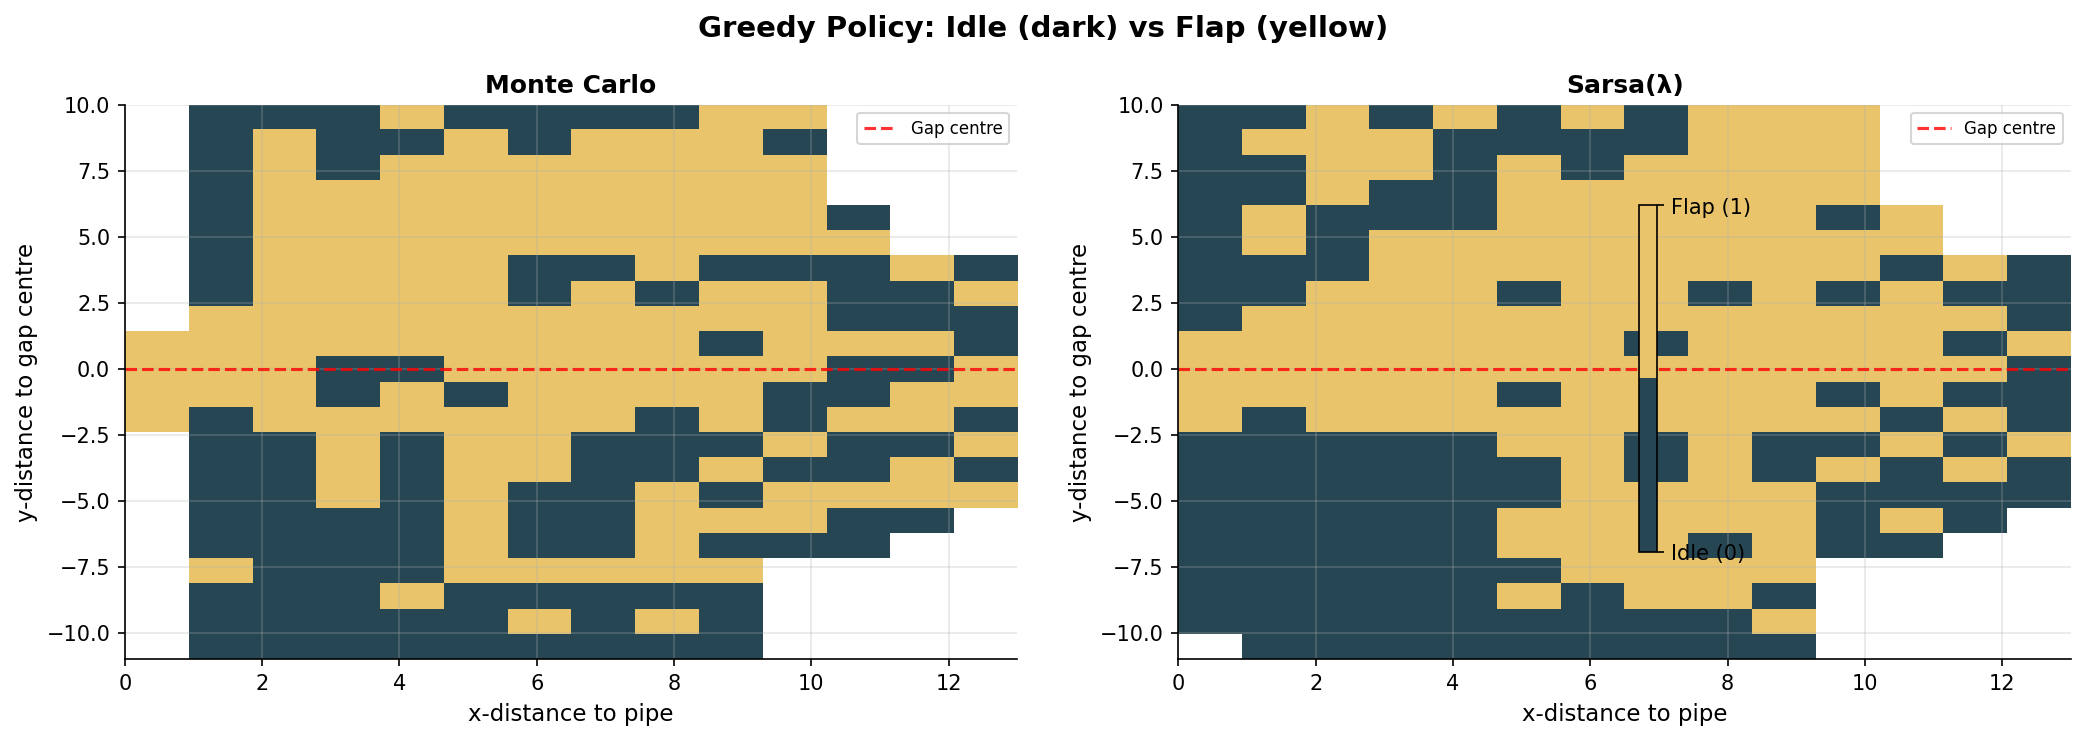
\includegraphics[width=\linewidth]{policies.png}
  \caption{Greedy policy maps (blue~=~flap, orange~=~idle).}
  \label{fig:policy}
\end{figure}

% ------------------------------------------------------------------
\section{Discussion}

\subsection*{Q1 — Algorithm comparison}

Table~\ref{tab:compare} summarises the key differences.
MC is simpler but slow: short early episodes provide little signal per
episode refresh.
Sarsa($\lambda$) bootstraps and spreads credit backwards at every step,
achieving both faster convergence and higher final performance.
Sensitivity-wise, MC is primarily sensitive to $\alpha$; Sarsa adds $\lambda$
as a critical parameter (see Sect.~\ref{sec:sweep}).

\begin{table}[H]
  \centering
  \caption{Agent comparison.}
  \label{tab:compare}
  \small
  \begin{tabular}{lcc}
    \toprule
    & \textbf{Monte Carlo} & \textbf{Sarsa($\lambda$)} \\
    \midrule
    Update timing     & End of episode    & Every step \\
    Bootstrapping     & No                & TD error \\
    Traces            & No                & $\lambda$-weighted \\
    States explored   & 271 / 308         & 298 / 308 \\
    Mean score (25k)  & 65.2 pipes        & \textbf{199.0 pipes} \\
    Key parameters    & $\alpha$          & $\alpha$, $\lambda$ \\
    \bottomrule
  \end{tabular}
\end{table}

\subsection*{Q2 — Two TFB environment versions}

\texttt{TextFlappyBird-v0} gives a compact 2D distance observation, yielding
308 discrete states — ideal for tabular methods.
\texttt{TextFlappyBird-screen-v0} returns the full ASCII screen render:
the state space grows exponentially with grid size (curse of dimensionality),
making tabular Q-tables intractable.
Use-case limitation: the compact version loses information on bird velocity
and multiple upcoming pipes; the screen version is faithful but requires function
approximation (e.g.\ DQN with a CNN).

\subsection*{Q3 — Original Flappy Bird}

The original \texttt{flappy-bird-gym}~\cite{talendar2021fbgym} uses continuous
physics (gravity, velocity) and pixel observations.
Tabular agents cannot scale to continuous or high-dimensional spaces without
discretisation.
In practice one would use \emph{tile-coding} for state aggregation, or a deep
agent such as DQN with frame stacking and convolutional feature extraction.

\subsection*{Q4 — Generalisation across configurations}
\label{sec:gen}

We trained both agents on the default config and evaluated them on an
alternative configuration (Fig.~\ref{fig:gen}; Table~\ref{tab:gen}).
Zero-shot transfer degrades performance sharply: a new config shifts the
$(x,y)$ state distribution, exposing unseen states whose Q-values default
to zero. Retraining Sarsa($\lambda$) from scratch on the new config recovers
near-perfect play (\textbf{249 pipes}).
This highlights the fundamental limitation of tabular agents: they memorise
state-action pairs and do not generalise across environment geometries.

\begin{table}[H]
  \centering
  \caption{Generalisation results (mean score / mean reward).}
  \label{tab:gen}
  \small
  \begin{tabular}{lcc}
    \toprule
    Condition & Score & Reward \\
    \midrule
    MC (default $\to$ alt)          & 12.0 & 106.3 \\
    Sarsa($\lambda$) (default$\to$alt) & 1.7  & 23.6  \\
    MC retrained on alt             & 4.9  & 48.1  \\
    Sarsa($\lambda$) retrained       & \textbf{249.0} & \textbf{2000.0} \\
    \bottomrule
  \end{tabular}
\end{table}

\begin{figure}[H]
  \centering
  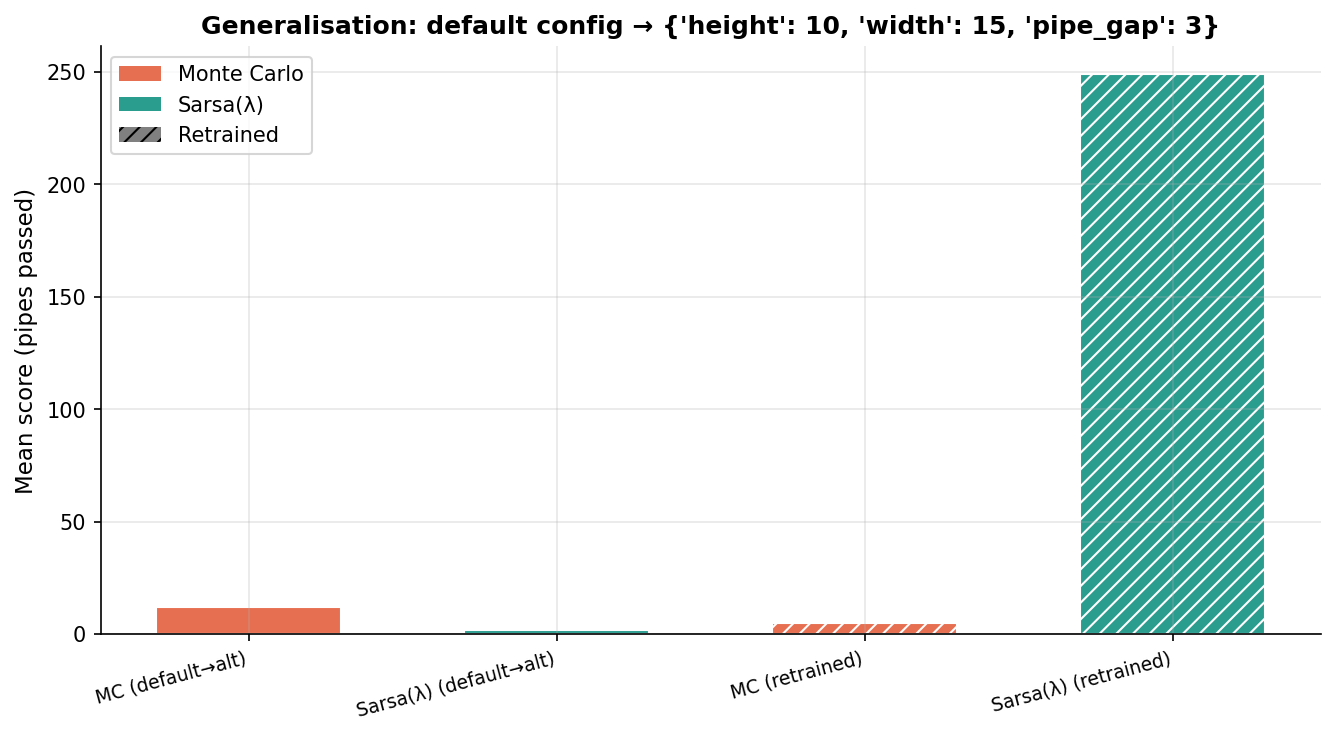
\includegraphics[width=0.85\linewidth]{generalisation.png}
  \caption{Generalisation: mean score across four conditions.}
  \label{fig:gen}
\end{figure}

\subsection*{Q5 — Parameter sensitivity}
\label{sec:sweep}

Figure~\ref{fig:sweep} shows sweeps over $\alpha$ and $\lambda$ (10\,000
episodes each).
\textbf{$\alpha$ sweep:} MC peaks at $\alpha=0.1$ (score 153.6 at 10k ep.);
Sarsa at $\alpha=0.2$ (score 199.0).
Very small $\alpha$ ($\leq$0.05) prevents convergence; large $\alpha$
($\geq$0.5) causes instability.
\textbf{$\lambda$ sweep:} Performance increases monotonically up to $\lambda=0.9$
(score 53.6 at 10k ep.) then drops slightly at $\lambda=0.99$ due to near-infinite
trace accumulation.
Both agents are fairly robust around their optimal values.

\begin{figure}[H]
  \centering
  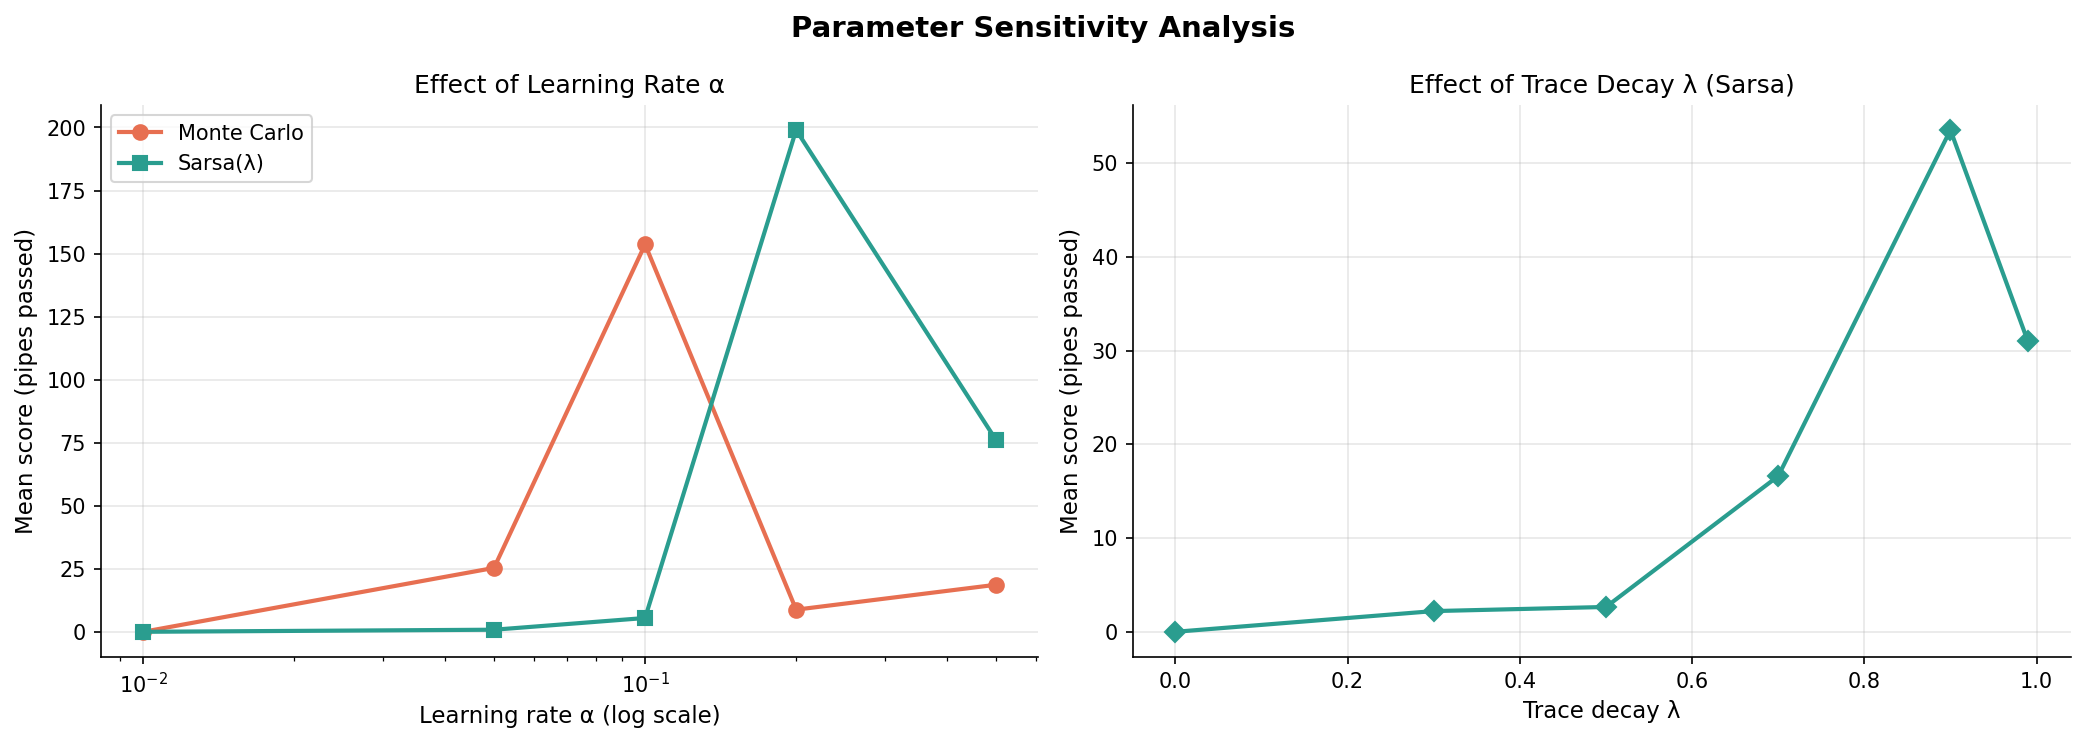
\includegraphics[width=\linewidth]{parameter_sweep.png}
  \caption{$\alpha$ sweep for both agents (left) and $\lambda$ sweep for
           Sarsa($\lambda$) (right) at 10\,000 training episodes.}
  \label{fig:sweep}
\end{figure}

% ------------------------------------------------------------------
\section{Conclusion}

Sarsa($\lambda$) substantially outperforms First-Visit MC on
\texttt{TextFlappyBird-v0} (199 vs.\ 65 mean pipes after 25\,000 episodes),
thanks to online, bootstrapped updates with eligibility traces.
Both agents are interpretable through their tabular Q-functions, but neither
generalises across environment configurations without retraining.
Future work could explore linear function approximation or DQN to handle
larger state spaces and enable configuration transfer.

\bigskip
\noindent\textbf{Code notebook:}
\url{https://github.com/YOUR_USERNAME/flappy-rl-assignment}
% <- replace with your actual Colab/GitHub link before submitting

% ------------------------------------------------------------------
\begin{thebibliography}{9}
\bibitem{sutton2018rl}
  R.~Sutton, A.~Barto:
  \emph{Reinforcement Learning: An Introduction}, 2nd edn.
  MIT Press (2018).

\bibitem{christodoulidis2023tfb}
  S.~Christodoulidis:
  Text Flappy Bird Gym. GitLab (2023).
  \url{https://gitlab-research.centralesupelec.fr/stergios.christodoulidis/text-flappy-bird-gym}

\bibitem{talendar2021fbgym}
  Talendar:
  Flappy Bird Gym. GitHub (2021).
  \url{https://github.com/Talendar/flappy-bird-gym}
\end{thebibliography}

\end{document}
